\qquad A análise de complexidade do Selection Sort, considerando as
diferentes situações de entrada (crescente, decrescente e
randômica), foi realizada manuscrita, com a devida justificativa,
contando o número de execuções de cada linha do algoritmo, no mesmo
formato adotado no capítulo anterior, conforme exigido pelo enunciado
do trabalho.

\begin{figure}[htbp]
    \centering
    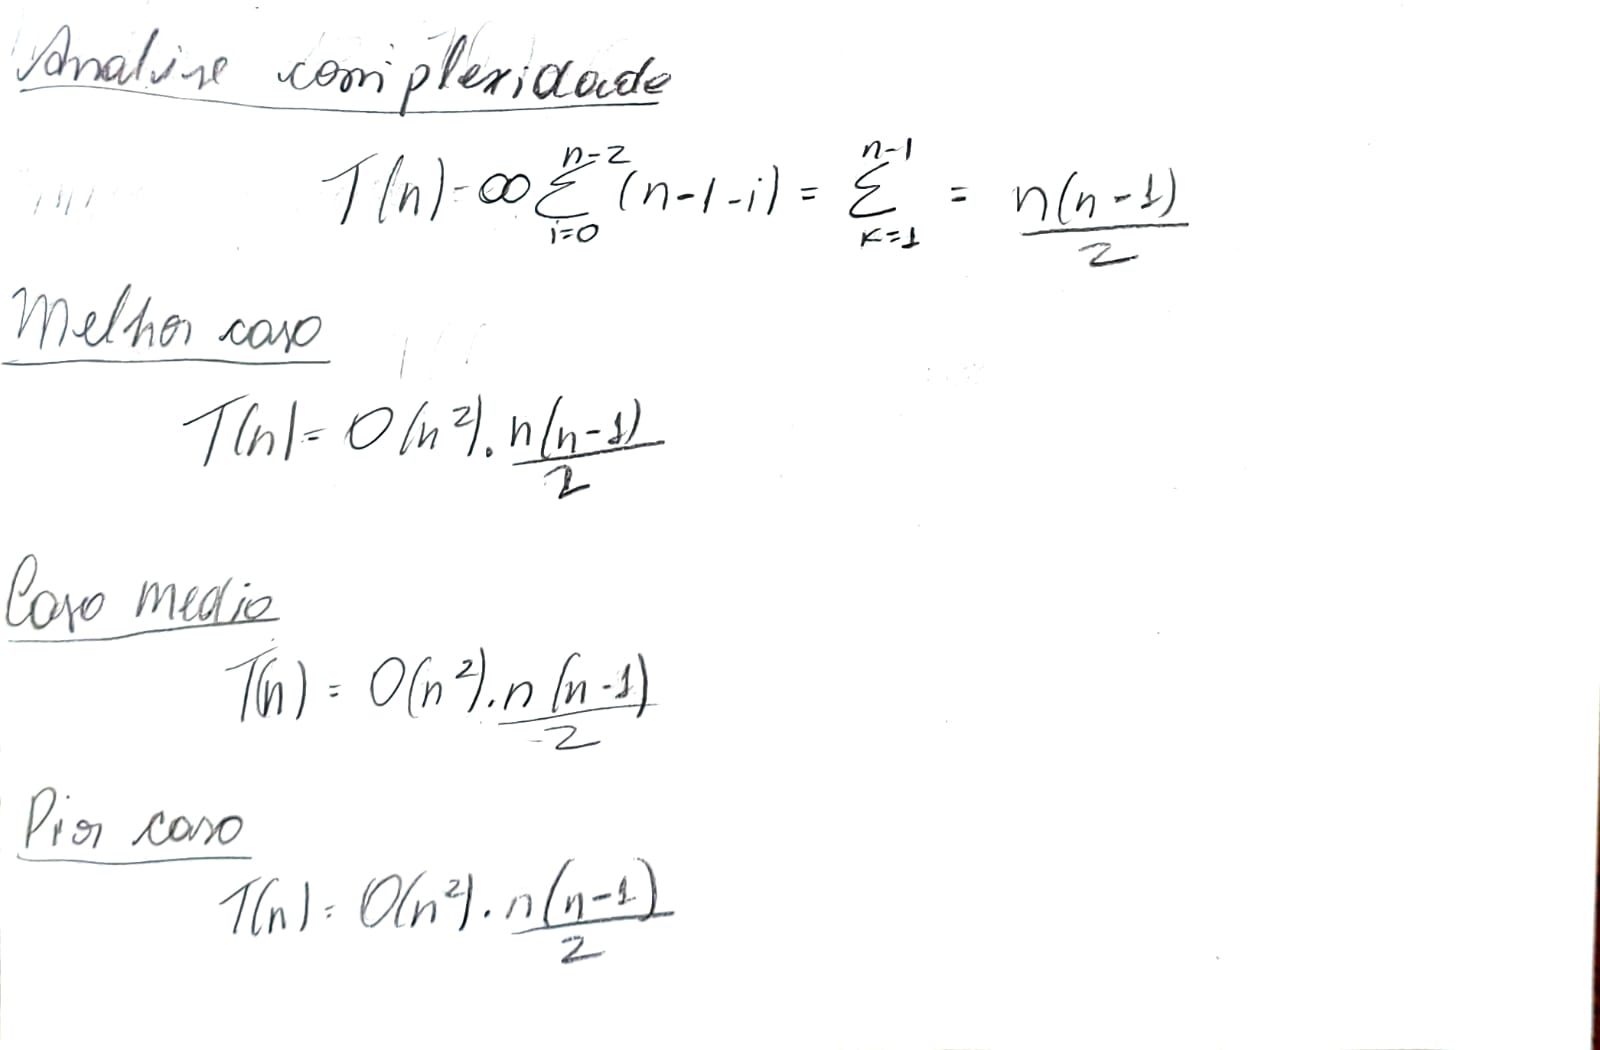
\includegraphics[width=14cm]{Imagens/Selection Sort/analise_complexidade.jpeg}
    \caption{Análise de complexidade manuscrita do algoritmo Selection Sort}
    \label{fig:analise_complexidade_selection}
\end{figure}

\qquad Diferentemente do Insertion Sort, o laço interno do Selection
Sort sempre percorre integralmente as posições restantes à procura do
menor elemento, independentemente da ordem dos dados. Por isso, os
três casos coincidem na mesma ordem de grandeza:

\textbf{Melhor caso (entrada crescente):} ainda assim são realizadas
$\sum_{i=0}^{n-2}(n-1-i) = \dfrac{n(n-1)}{2}$ comparações; nenhuma
troca é necessária, mas o número de comparações já garante
$T(n) = \Theta(n^2)$.

\textbf{Caso médio (entrada randômica):} o número de comparações
permanece $\frac{n(n-1)}{2}$; o número esperado de trocas passa a ser
da ordem de $n$ (bem menor que o número de comparações), mantendo
$T(n) = \Theta(n^2)$.

\textbf{Pior caso (entrada decrescente):} o número de comparações
continua $\frac{n(n-1)}{2}$ e o número de trocas atinge seu máximo,
$n-1$; como esse termo é linear e as comparações são $\Theta(n^2)$, o
termo quadrático domina e $T(n) = \Theta(n^2)$.

\qquad Ou seja, ao contrário do Insertion Sort e do Bubble Sort, no
Selection Sort os três casos (melhor, médio e pior) têm exatamente a
mesma ordem de grandeza, $\Theta(n^2)$, pois o número de comparações
não depende do tipo de entrada — apenas o número de trocas (sempre
$O(n)$, desprezível diante das comparações) varia. Os resultados
experimentais apresentados na próxima seção confirmam essa previsão
teórica: os tempos medidos para entradas crescente, decrescente e
randômica são praticamente idênticos entre si, para um mesmo tamanho
de instância.
